\chapter{The CALIFA survey}

In this chapter we present an overview of the CALIFA survey, including several generalities concerning the CALIFA datasets. In
particular, we discuss the selection criteria of the galaxies relevant to this work. In addition,
 a brief description of the two different configurations available for CALIFA data is presented.

\section{The CALIFA survey}

The CALIFA survey is a comprehensive wide field  integral field unit (IFU) survey carried out in the Calar Alto observatory in
Almer\'ia, Spain. It is operated jointly with the Max Plank Insititut f\"{u}r Astronomie and the Instituto de Astrof\'isica de
Andaluc\'ia. Obervations began in June of 2010, with the survey collecting data from over six hundred galaxies in two configurations,
the V500 and the V1200 set ups [4] described in the following section.

%\begin{figure}
%  \centering
%  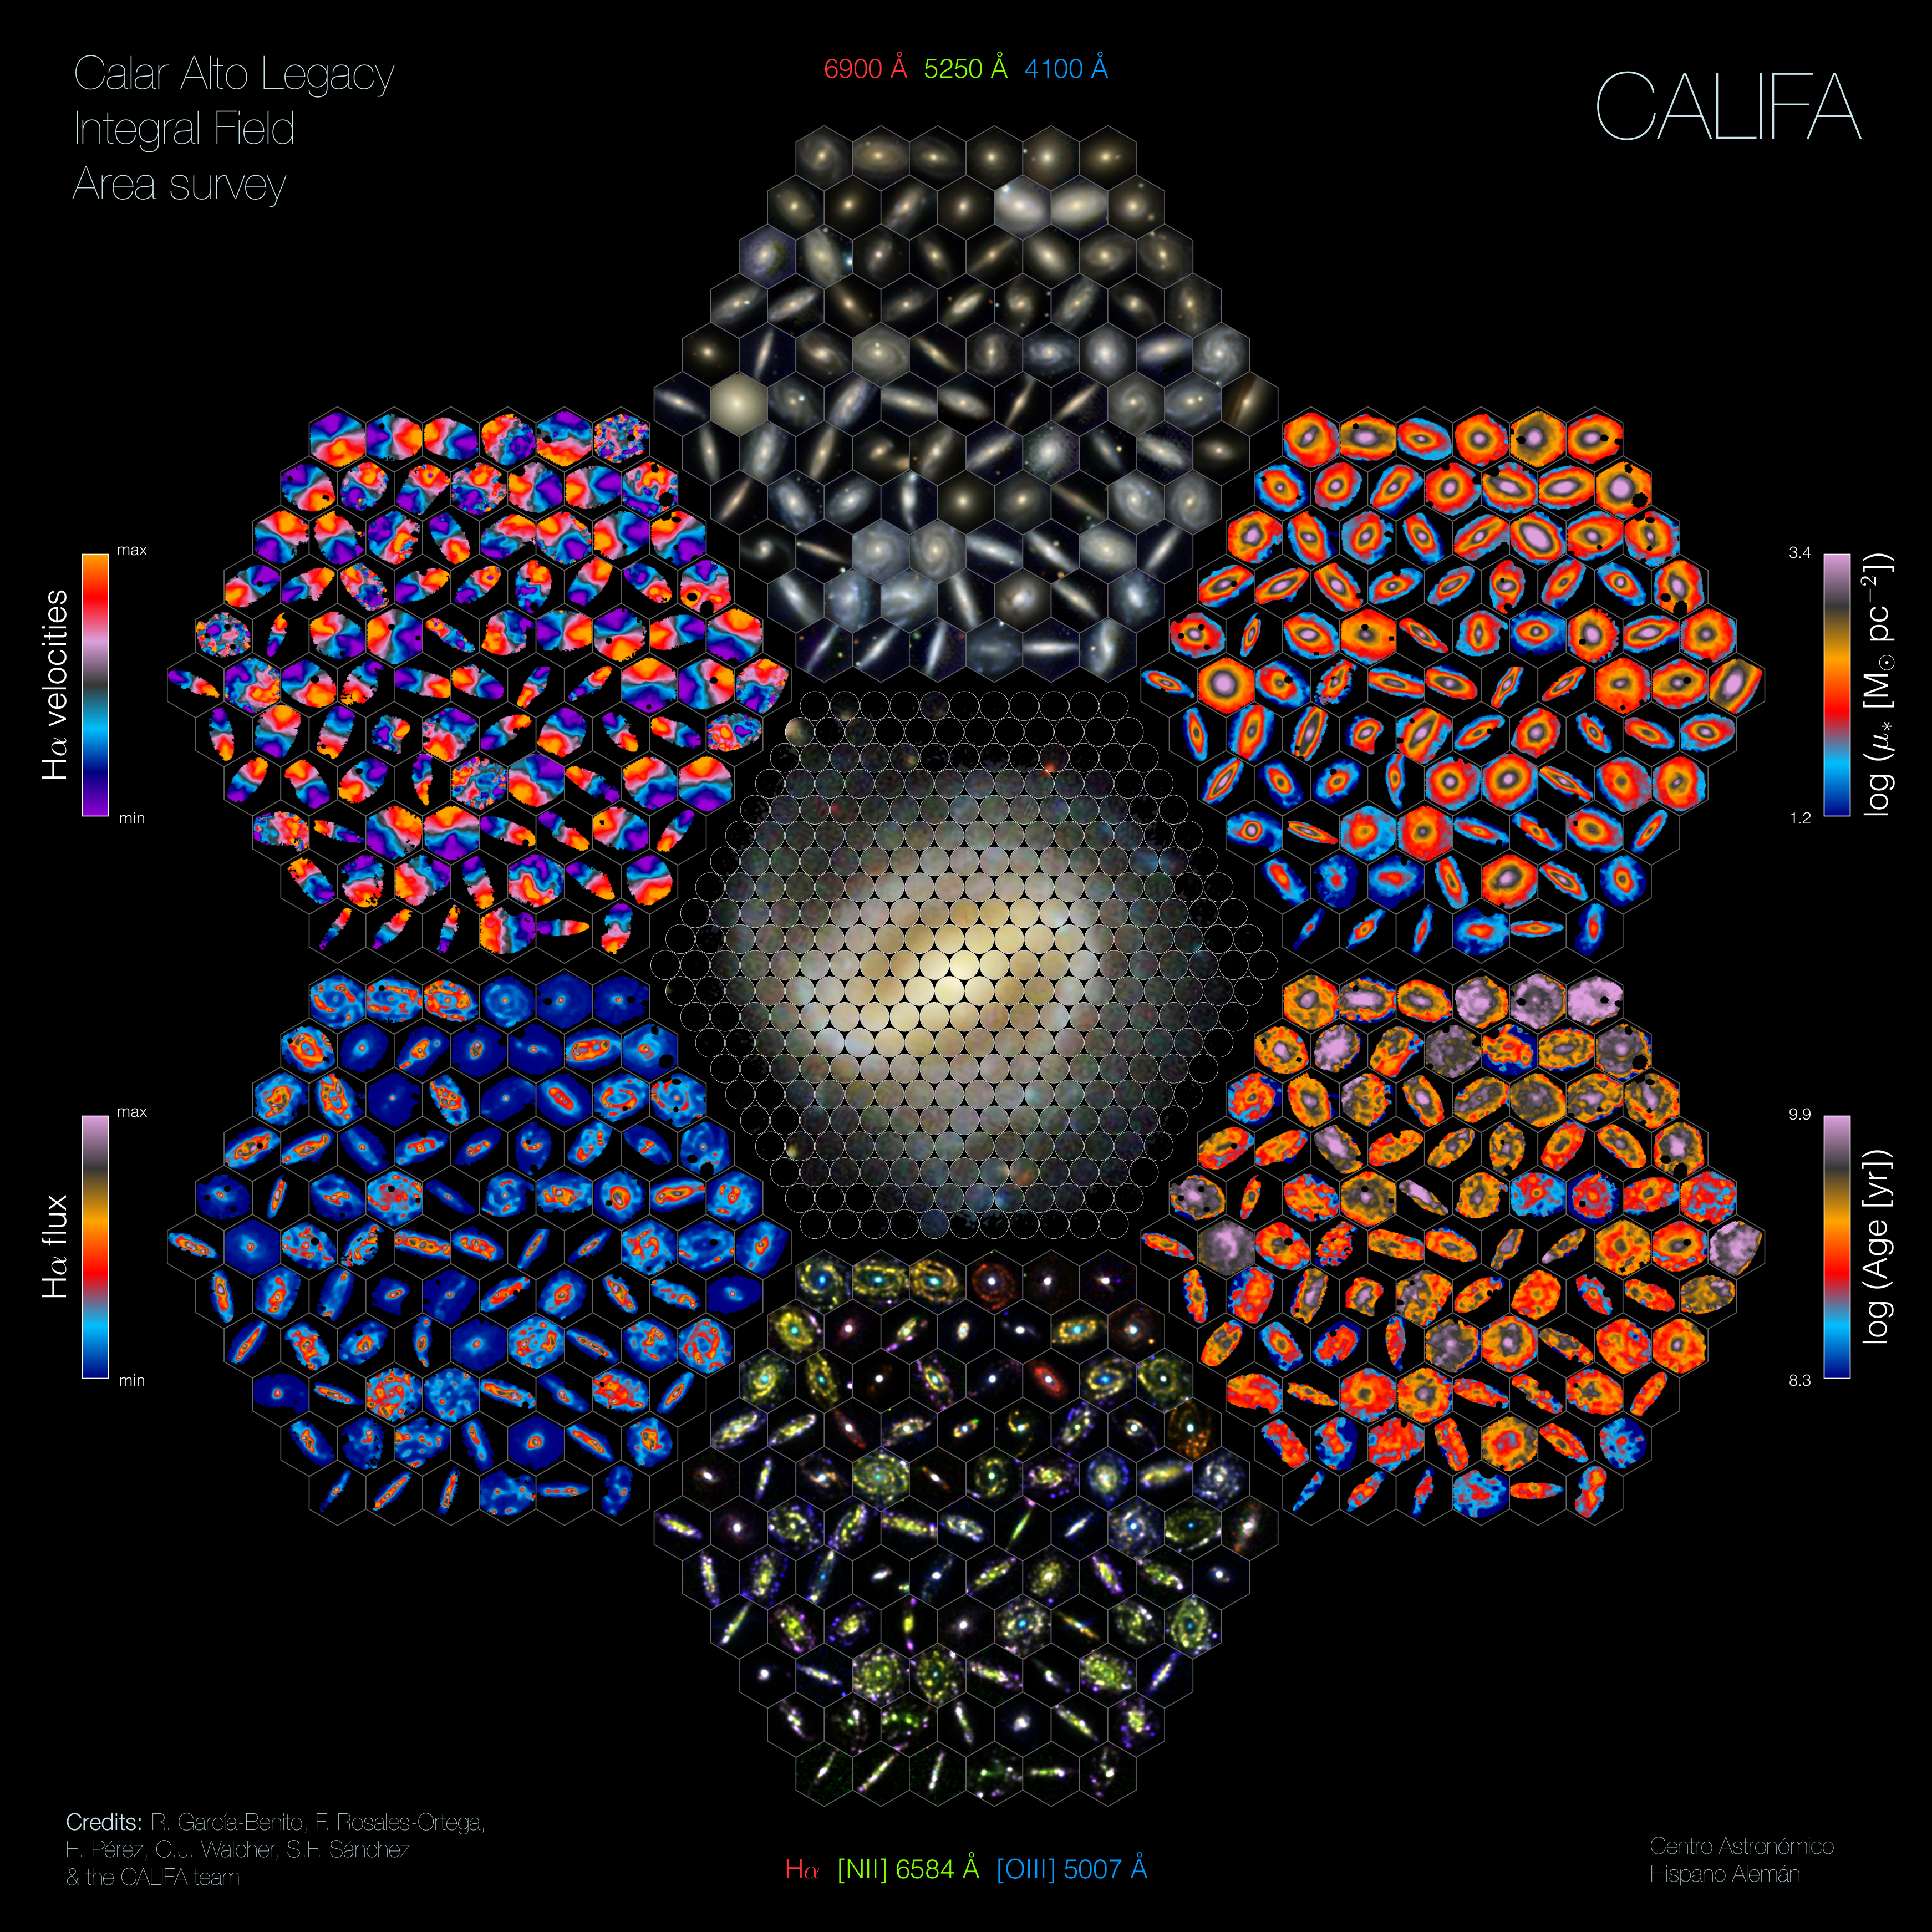
\includegraphics[scale=0.2]{califa.jpg}
%  \caption{http://califaserv.caha.es/CALIFA/DATA/Figs/CALIFA$\_$HexRGB.jpg}
%  \label{fig2:1}
%\end{figure}

The reasoning for selecting CALIFA survey data is simple. As seen in figure \ref{fig2:1}, CALIFA data does not consists of a single
spectra, instead, multiple optic fibers were pointed at a single galaxy [4, 5]. For previous surveys having a single measure of a
spectra meant that for an entire galaxy there was only one reported value of total SFR. Since stochasticity theoretically appears
in low SFR regions, the ability to focus on distinct regions that have lower SFR opens the possibility of searching for this
stochastic effects.

In this work, we will be using ``face on" galaxies from the CALIFA catalog published in [6]. These type of galaxies are optimal
for a complete scanning and allow us to measure the spectra of individual regions within a galaxy.
We did a manual selection of the datacubes in [6] to select galaxies whose galactic planes are
perpendicular to our field of view.

\section{The CALIFA datacubes}

The CALIFA datacubes consist of a three dimensional array, where the $x$ and $y$ coordinates indicate the right ascension and
declination of the target, and the $z$ axis contains information about flux intensity and wavelength of that pixel along with the
error associated with those fluxes, a mask to cover bad pixels and the covariance weight of the error propagation [4, 5].

The V500 and V1200 configurations cover different wavelength intervals and have different resolution, with the V500 datacube having
a resolution of $^{\lambda}/_{\Delta \lambda} \sim 850$ and covering emission lines between $3745 - 7500$ \AA, while the V1200
configuration has a higher resolution of $^{\lambda}/_{\Delta \lambda} \sim 1650$ and compiles wavelengths from $3700 - 4800$ \AA.
$\left[4, 5\right]$

In this work, we will be using the lower resolution V500 datacubes published in [6] which have been subjected to the Pipe3D analysis
pipeline explained in section 3.2 and detailed in [6]. These datacubes contain a great deal of information, including that of
intermediate steps of the fitting procedure.
